% \vspace{-0.5em}
\section{Method}
\label{sec:method}
% \vspace{-0.5em}
\paragraph{Background and notation}
The system's commonsense knowledge is a KB, denoted \KB, programmed in a Prolog-like syntax.
% In this paper, we use a knowledge base, denoted with \KB, to do reasoning. \KB~is programmed in a Prolog-like syntax.
% As stated, our knowledge base is programmed in a prolog-like syntax. 
We have developed a modified version of Prolog, which has been augmented to support several special features (types, soft-matched predicates and atoms, etc). %required for addressing the challenges discussed in the next sub-section.  %knowledge misalignment problem $\mathfrak{C}.2$. 
% \begin{table*}[t]
    \caption{Different reasoning templates of the statements that we uncovered, presumably reflecting how humans logically reason. $\wedge$, $\neg$, $\coloneq$ indicate logical and, negation, and implication, respectively. $\textAction_h$ is an action that is hidden in the main utterance and $\textAction(\textState)$ indicates performing the $\textAction$ when the $\textState$ holds.}
    \label{tab:logic_templates}
\centering
\resizebox{0.9\textwidth}{!}{%
    \begin{tabular}{llc}
        \toprule 
        \bf{Logic template} & \textbf{Example} & \bf{Count} \\
        \midrule
        1. \thead[l]{\blueTemplate{$(\neg(\text{\textGoal}) \coloneq \text{\textState}) \wedge$} \\ \blueTemplate{$(\text{\textGoal} \coloneq \text{\textAction}(\text{\textState}))$}} & \thead[l]{If it snows tonight \\ then wake me up early \\ because I want to arrive to work on time} & 65 \\
        % &  &\\
        2. \thead[l]{\orangeTemplate{$(\text{\textGoal} \coloneq \text{\textAction}(\text{\textState})) \wedge$} \\ \orangeTemplate{$(\neg(\text{\textGoal}) \coloneq \neg(\text{\textAction}(\text{\textState})))$}} & \thead[l]{If I am walking to a meeting \\ then remind me who else is there \\ because I want to be prepared for the meeting} & 50 \\
        % & &\\
        3. \thead[l]{\greenTemplate{$(\text{\textGoal} \coloneq \text{\textAction}_h) \wedge$} \\ \greenTemplate{$(\text{\textAction}_h \coloneq \text{\textAction}(\text{\textState}))$}} & \thead[l]{If we are approaching Fall \\ then remind me to buy flower bulbs \\ because I want to make sure I have a pretty Spring garden.} & 17 \\
        % & &\\
        4. \thead[l]{\purpleTemplate{$(\text{\textGoal} \coloneq \text{\textState}) \wedge$} \\  \purpleTemplate{$(\neg(\text{\textGoal}) \coloneq \text{\textAction}(\text{\textState}))$}}
        & \thead[l]{If I am at the grocery store but I have a trip coming up in the next week \\ then remind me not to buy perishables \\ because they will go bad while I am away} & 5 \\
        % & & \\
        % 5. \thead[l]{\pinkTemplate{$(\text{\textState} \coloneq \text{\textAction}) \wedge$} \\ \pinkTemplate{$(\text{\textAction} \coloneq \text{\textGoal})$}} & \thead[l]{If I schedule an appointment that overlaps with another appointment \\ then notify me immediately \\ because I want to notify my colleagues of the conflict.} & 1 \\
        % & & \\
        5. \redTemplate{other} & \thead[l]{If tomorrow is a holiday \\ then ask me if I want to disable or change my alarms \\ because I don't want to wake up early if I don't need to go to work early.}  &23 \\
        \bottomrule
    \end{tabular}
    }
\end{table*}
% As stated, we assume that CORGI has access to a small amount of background knowledge, $K$. %Amos: if we need extra space the two previous sentence can be removed. In general most of this subsection may be removed or shortened if we don't have space.
% In our study, $K$ consists of logical facts and rules programmed in Prolog. Prolog is a declarative logic programming language consisting of relations, which are a generalization of functions in functional programming. We have developed a modified version of Prolog, which has been augmented to support several special features (types, soft-matched predicates and atoms, etc) required by our model.
Prolog \cite{colmerauer1990introduction} is a declarative logic programming language that consists of a set of predicates whose arguments are atoms, variables or predicates. A predicate is defined by a set of rules (\prologTerm{$\text{Head} \coloneq \text{Body}.$}) and facts (\prologTerm{$\text{Head}.$}), where \prologTerm{Head} is a predicate, \prologTerm{Body} is a conjuction of predicates, and \prologTerm{$\coloneq$} is logical implication. We use the notation $\state$, $\action$ and $\goal$ to represent the logical form of the \textState, \textAction and \textGoal, respectively where $S$, $A$ and $G$ are predicate names and $X, Y$ and $Z$ indicate the \emph{list} of arguments of each predicate. For example, for \textGoal=``I want to get to work on time'', we have $\goal=$\prologTerm{get(i, work, on\_time)}. Prolog can be used to logically ``prove'' a query (e.g., to prove $\goal$ from $S(X), G(Z)$ and appropriate commonsense knowledge (see the Appendix - Prolog Background)).
%%% if you want the prolog subsection back uncomment the following
% % In Prolog, all the data including a Prolog program are represented as Prolog terms. \amoscomment{can you please rephrase the previous sentence? Or maybe remove it.}
% Prolog \cite{colmerauer1990introduction} is a declarative logic programming language. A Prolog program consists of a set of predicates. A predicate has a name (functor) and $N\geq0$ arguments. $N$ is referred to as the arity of the predicate. A predicate with functor name $F$ and arity $N$ is represented as $F(T_1, \dots, T_N)$ where $T_i$'s, for $i\in [1,N]$, are the arguments that are arbitrary Prolog terms. A Prolog term is either an atom, a variable or a compound term (a predicate with arguments). A variable starts with a capital letter (e.g., \prologTerm{Time}) and atoms start with small letters (e.g. \prologTerm{monday}). We use the notation $\state$, $\action$ and $\goal$ to represent the logical form of the \textState, \textAction and \textGoal, respectively where $S$, $A$ and $G$ are predicate names and $X, Y$ and $Z$ indicate the \emph{list} of arguments of each predicate. We refrained from expanding the argument list for these predicates to make the notation more compact.
% % The predicate name is an atom and each argument is an arbitrary Prolog term.
% A predicate defines a relationship between its arguments. For example, \prologTerm{isBefore(monday, tuesday)} indicates that the relationship between Monday and Tuesday is that, the former is before the latter.

%A predicate is defined by a set of clauses. A clause is either a Prolog~~\emph{fact} or a Prolog \emph{rule}. A Prolog rule is denoted with \prologTerm{$\text{Head} \coloneq \text{Body}.$} and a fact is a rule whose body is \prologTerm{True}.
% % \begin{equation}
% %     \text{Head} \coloneq \text{Body}.
% % \end{equation}
% where the \prologTerm{Head} is a predicate, the \prologTerm{Body} is a conjunction (\prologTerm{$\wedge$}) of predicates, \prologTerm{$\coloneq$} is logical implication, and period indicates the end of the clause. The previous rule is an if-then statement that reads ``\emph{if} the Body holds \emph{then} the Head holds''.
% %The Body of the rule is also referred to as the rule goal. %If the body of the rule holds then the head of the rule holds as well.
% A fact is a rule whose body always holds, and is indicated by \prologTerm{Head.} 
% % \begin{equation}
% %     Head.
% % \end{equation}
% , which is equivalent to \prologTerm{Head $\coloneq$  true.}
% % \begin{equation}
% %     \text{Head} \coloneq true.
% % \end{equation}

% Prolog can be used to logically ``prove'' whether a specific query holds or not (For example, to prove that \prologTerm{isAfter(wednesday,thursday)?} is \prologTerm{false}). The proof is performed through \emph{backward chaining}, which is a backtracking algorithm that usually employs a depth-first search strategy. At the heart of backward chaining is the \emph{unification} operator, which matches the arguments of a query and a rule's head.
% A detailed explanation of backward chaining and unification is provided in the Appendix. 
% \vspace{-0.5em}
\subsection{CORGI: COmmonsense Reasoning by Instruction}
\label{sec:corgi}
CORGI takes as input a natural language command of the form ``if $\langle$\textState$\rangle$ then $\langle$\textAction$\rangle$ because $\langle$\textGoal$\rangle$'' and infers commonsense presumptions by extracting a chain of commonsense knowledge that explains how the commanded \textAction achieves the \textGoal when the \textState holds. For example from a high level, for the command in Fig.~\ref{fig:prooftree} CORGI outputs $(1)$ if it snows more than two inches, then there will be traffic, $(2)$ if there is traffic, then my commute time to work increases, $(3)$ if my commute time to work increases then I need to leave the house earlier to ensure I get to work on time $(4)$ if I wake up earlier then I will leave the house earlier. Formally, this reasoning chain is a proof tree (proof trace) shown in Fig.\ref{fig:prooftree}. 
% (also see Fig.\ref{fig:prooftree_simple}). 
% This reasoning chain is obtained by logically proving the \textGoal against a knowledge base $K$.
% We refer to this reasoning chain as a proof trace (or proof tree). Formally, the proof trace of the above reasoning chain is shown in Fig.\ref{fig:prooftree}. 
As shown, the proof tree includes the commonsense presumptions.% that humans would make when encountering the input statement. %In what follows we explain the details of how this is done in CORGI.

CORGI's architecture is depicted in Figure \ref{fig:model}. In the first step, the if-then-because command goes through a parser that extracts the \textState, \textAction and \textGoal from it and converts them to their logical form representations $\state$, $\action$ and $\goal$, respectively.
% that consist of a predicate name and a set of arguments. 
For example, the \textAction ``wake me up early'' is converted to \prologTerm{wake(me, early)}. The parser is presented in the Appendix (Sec. Parsing). %. CORGI then parses the utterance and converts the \textState, \textAction and \textState to their corresponding logical forms $\state$, $\action$ and $\goal$, respectively. 

% Using a small amount of background commonsense knowledge, CORGI ``reasons'' about the input statement by logically proving $\goal$. The proof is a multi-hop reasoning chain of commonsense knowledge that indicates how performing the \textAction allows one to achieve the \textGoal when the \textState holds (refer to the introduction for an example and Figure \ref{fig:prooftree_simple}). Therefore we have
The proof trace is obtained by
finding a proof for $\goal$, using 
% background commonsense knowledge base, 
\KB~and the context of the input if-then-because command. In other words, $\state \cap \action \cap K \rightarrow \goal.$
% \begin{equation}
%     \state \cap \action \cap K \rightarrow \goal.
% \end{equation}
One challenge is that even the largest knowledge bases gathered to date are incomplete, making it virtually infeasible to prove an arbitrary input $\goal$. Therefore, CORGI is equipped with a conversational interaction strategy, which enables it to prove a query by combining its own commonsense knowledge with conversationally evoked knowledge provided by a human user in response to a question from CORGI (\emph{user feedback loop} in Fig.\ref{fig:model}).
% extracts missing knowledge from a human user by conversing with them (\emph{user feedback loop} in Fig.\ref{fig:model}). 
There are 4 possible scenarios that can occur when CORGI asks such questions:
\vspace{-0.5em}
\begin{itemize}%[leftmargin=2em]
    \item[$\mathfrak{A}$] The user understands the question, but does not know the answer.
    \vspace{-0.4em}
    \item[$\mathfrak{B}$] The user misunderstands the question and responds with an undesired answer.
    \vspace{-0.4em}
    \item[$\mathfrak{C}$] The user understands the question and provides a correct answer, but the system fails to understand the user due to:
    \vspace{-0.4em}
    \begin{itemize}
        \item[$\mathfrak{C}.1$] limitations of natural language understanding.
        \vspace{-0.2em}
        \item[$\mathfrak{C}.2$] variations in natural language, which result in misalignment of the data schema in the knowledge base and the data schema in the user's mind.
    \end{itemize}
    \vspace{-0.5em}
    \item[$\mathfrak{D}$] The user understands the question and provides the correct answer and the system successfully parses and understands it.
\end{itemize}
\vspace{-0.5em}
\CORGI's different components are designed such that they address the above challenges, as explained below.
% CORGI's design is deriven by the above observations. 
% and is developed to address the challenges of the above scenarios. 
Since our benchmark data set deals with day-to-day activities, it is unlikely for scenario $\mathfrak{A}$ to occur. If the task required more specific domain knowledge, $\mathfrak{A}$ could have been addressed by choosing a pool of domain experts. Scenario $\mathfrak{B}$ is addressed by asking informative questions from users. 
Scenario $\mathfrak{C}.1$ is addressed by trying to extract small chunks of knowledge from the users piece-by-piece. Specifically, the choice of what to ask the user in the \emph{user feedback loop} is deterministically computed from the user's \textGoal. The first step is to ask how to achieve the user’s stated \textGoal, and CORGI expects an answer that gives a sub-\textGoal. In the next step, CORGI asks %Amos how about "the next step is to ask"? or "in the next step CORGI asks" Forough: fixed
how to achieve the sub-\textGoal the user just mentioned. 
% This design choice is to address limitation $\mathfrak{C}.1$. 
The reason for this piece-by-piece knowledge extraction is to ensure that the language understanding component can correctly parse the user's response. CORGI then adds the extracted knowledge from the user to \KB~in the \emph{knowledge update loop} shown in Fig.\ref{fig:model}. Missing knowledge outside this \textGoal/sub-\textGoal path is not handled, although it is an interesting future direction. Moreover, the model is user specific and the knowledge extracted from different users are not shared among them. Sharing knowledge raises interesting privacy issues and requires handling personalized conflicts and falls out of the scope of our current study.
% As the natural language processing community makes more progress, this will be less of a limitation in a model that learns through coversational interactions. 

Scenario $\mathfrak{C}.2$, caused by the variations of natural language, results in semantically similar statements to get mapped into different logical forms, which is unwanted. For example, ``make sure I am awake early morning'' vs. ``wake me up early morning'' will be parsed into different logical forms \prologTerm{awake(i,early$\_$morning)} and \prologTerm{wake(me, early$\_$morning)},
respectively although they are semantically similar. This mismatch prevents a logical proof from succeeding since the proof strategy relies on exact match in the unification operation (see Appendix). This is addressed by our neuro-symbolic theorem prover (Fig.\ref{fig:model}) that learns vector representations (embeddings) for logical rules and variables and uses them to perform a logical proof through soft unification. If the theorem prover can prove the user's \textGoal, $\goal$, CORGI outputs the proof trace (Fig.\ref{fig:prooftree}) returned by its theorem prover and succeeds. In the next section, we explain our theorem prover in detail.
\begin{figure*}\centering
\newcommand{\anonvar}{\rule{0.7em}{0.4pt}}
\newcommand{\rbox}[2]{\parbox{#1}{
\raggedright
\hangindent=1.5em
\hangafter=1
#2}}
\newlength{\pushdown}
\setlength{\pushdown}{0.5cm}

\resizebox{0.9\textwidth}{!}{%
%
\begin{tikzpicture}
[level distance=1.1cm,
    level 1/.style={sibling distance=7cm},
    level 2/.style={sibling distance=5cm},
    level 3/.style={sibling distance=4cm},
proofstep/.style={rectangle,draw=black,inner sep=4pt}]
\node [proofstep, label=left:{$t=0$}, fill=lavendergray] (get) {get(Person, ToPlace, on$\_$time)}
child { node [proofstep,left=-2cm, label=left:{$t=1$}] (arrive) {arrive(Person, \anonvar, \anonvar, ToPlace, ArriveAt)}
    child { node [proofstep, fill=celadon, label=left:{$t=2$}] (ready) {ready(Person, LeaveAt, PrepTime)}
        child { node [proofstep, fill=celadon, label=left:{$t=3$}, left=0.2cm] (alarm) {alarm(Perosn, Time)} child{node [proofstep, label=left:{$t=4$}] (ground_alarm) {alarm(i,8)} } }
        child { node [proofstep,below left=\pushdown and -2.2cm, fill=celadon, label=left:{$t=5$}] (leaveat) {LeaveAt = Time + PrepTime.}}
    }
    child { node [proofstep,below right=2.5cm and -2.5cm, label=left:{$t=6$}] (commute) {\rbox{5cm}{commute(Person, FromPlace, ToPlace, With, CommuteTime)}}
        child { node [proofstep,below=-0.3cm, label=left:{$t=7$}] (commutex) {commute(i, home, work, car, 1)} }
    }
    child { node [proofstep,below right=2.8cm and 0.5cm, label=left:{$t=8$}] (traffic) {\rbox{5cm}{traffic(LeaveAt, ToPlace, With, TrTime)}} 
        child { node [proofstep,below left=1\pushdown and -1cm, label=left:{$t=9$}] (weather) {weather(snow, Precipitation)} }
        child { node [proofstep,below right=1\pushdown and -0.6cm, fill=atomictangerine, label=left:{$t=10$}] (precipitation) {Precipitation $>=$ 2} }
        child { node [proofstep,below right=1\pushdown and 1cm, label=left:{$t=11$}] (travelTime) {TrTime = 1} }
    }
    child { node [proofstep,below right=2.5\pushdown and 0, label=left:{$t=12$}] (arriveat) {\rbox{5cm}{ArriveAt = LeaveAt + CommuteTime + TrTime}} }
}
child { node [proofstep, label=left:{$t=13$}] (cal) {calendarEntry(Person, ToPlace, ArriveAt)}
    child { node [proofstep, fill=atomictangerine, label=left:{$t=14$}] (calx) {calendarEntry(i, work, 9)} }
};
\end{tikzpicture} 
}
%Amos: can this figure appear a little bit earlier (closer to where it is called in text)?
    \caption{Sample proof tree for the \emph{because}-clause of the statement: ``If it snows tonight then wake me up early because I want to get to work on time''. Proof traversal is depth-first from left to right ($t$ gives the order). Each node in the tree indicates a rule's head, and its children indicate the rule's body. For example, the nodes highlighted in green indicate the rule \prologTerm{ready(Person,LeaveAt,PrepTime) $\coloneq$ alarm(Person, Time) $\wedge$ LeaveAt = Time+PrepTime}. The \textGoal we want to prove, $\goal$=\prologTerm{get(Person, ToPlace, on$\_$time)}, is in the tree's root. If a proof is successful, the variables in $\goal$ get grounded (here \prologTerm{Person} and \prologTerm{ToPlace} are grounded to \prologTerm{i} and \prologTerm{work}, respectively). The highlighted orange nodes are the uncovered commonsense presumptions.}
    \label{fig:prooftree}
    \vspace{-1em}
\end{figure*}
%\facomment{add a figure for the proof tree}
% Proof is performed using backward chaining, a backtracking algorithm implemented recursively. In each step of the recursion, the input is a goal to prove and the output is the proof's success/failure. in order to prove a query, a rule or fact whose head unifies with the query is retrieved from \KB. The proof continues recursively for each predicate in the body and succeeds if all the statements in the body of a rule are \prologTerm{true}. The base case (leaf) is when a fact is retrieved from \KB.
% \tmcomment{remove the left-to-right if it is not }
We revisit scenarios $\mathfrak{A}-\mathfrak{D}$ in detail in the discussion section and show real examples from our user study. 
% ``if the weather is snowy tonight'' vs. ``if the forecast calls for snow tonight'' will be parsed into different predicates \prologTerm{weather(snowy, tonight)} and \prologTerm{forecast(snow, tonight)},
% These different surface forms result in a failure of proof extraction in a hard logic theorem prover. In order to address this, our neuro-symbolic theorem prover learns vector representations or embeddings for logical rules and facts. 
% In the second step, CORGI attempts to prove the \textGoal by submitting a query to its neuro-symbolic theorem prover. If the proof succeeds, CORGI outputs a proof trace (Fig.\ref{fig:prooftree} shows an example) that uncovers the commonsense presumptions in the utterance.

% the model moves on to the next input. If the proof fails, it means $K$ has missing knowledge, therefore CORGI initiates a dialog with the user and tries to extract the missing knowledge required to prove the \textGoal, from the user (\emph{user feedback loop} in Fig.~\ref{fig:model}). The extracted knowledge will be added to CORGI's knowledge base in the \emph{knowledge base update loop} shown in Fig.~\ref{fig:model}, resulting in knowledge base completion. In the end, CORGI succeeds if a \emph{proof} is returned in the last step.

% We use the terminology $\state$, $\action$ and $\goal$ to refer to the logic representation of the \textState, \textAction and \textGoal as will be discussed in detail in the next subsection. The statement can then be read as: if \textState $\state$ is true, then perform \textAction $\action$ because I want to achieve \textGoal $\goal$.
% Moreover, we assume that we have access to a small amount of background knowledge,  $K$, that we will use to reason about the given statements. Our background knowledge is a collection of logical facts and rules programmed in a Prolog-like syntax.
% Commonsense reasoning in this paper is addressed by ``proving'' the \textGoal $\goal$ against the system's background knowledge $K$ such that the \textState $\state$ and \textAction $\action$ are in the proof trace.
% \begin{equation}
%     S(X) \wedge A_\theta(X) \wedge K \rightarrow G_\theta(X)
% \end{equation}
% where $K$ is the system's background knowledge.
% The returned proof trace includes the hidden presumptions in a given if-then-because utterance as explained in the Introduction section and shown in Fig.~\ref{fig:prooftree}. CORGI's flowchart is depicted in Fig.~\ref{fig:model}.

% Let us start by introducing some notations and background.
% Before we go deeper into the proposed model, let us start with a brief description of the background and notation.

% For example, the reasoning path for the example ``If it snows at night then wake me up early because I want to get to work on time.'' is %Amos: we can save some space here if needed.

% \begin{itemize}
%     \item[1] if it snows more than 2 inches, then there will be traffic
%     \item[2] if there is traffic then my commute time to work increases
%     \item [3] if my commute time to work increases then i need to leave the house earlier to get to work on time
%     \item[4] I will leave the house earlier if I wake up earlier.
% \end{itemize}

% Our goal is to find such a reasoning path for an input statement given the knowledge base and through engaging in a conversation with the user. In the above example, CORGI might already know items 1, 2 and 4 and not know how snow is relevant to getting on time to work. In this case, CORGI will ask the user how getting to work on time is relevant to the snow and hope to extract statement 3 from the user.

% \amoscomment{It is not clear to me which of the above items come from the system's background knowledge and which come from other sources.} % addressed

% ``If it snows at night then wake me up early because I want to see the snow.'' is
% \begin{itemize}
%     \item[1] if it snows, then the snow will cover the ground
%     \item[2] if snow is on the ground and it is not snowing, the snow will melt
%     \item [3] If I am awake before the snow melts then I will be able to see the snow
% \end{itemize}

% achieving the goal ``staying dry'' is:
% \amoscomment{It would be better to provide a full example, or maybe sticking with the previous example (``if it is snowing wake me up early so that I arrive on time to work") and showing how to achieve the goal of arriving on time to work} % good point I have used the same example now
% \begin{itemize}
%     \item[1] if the weather is bad, then it is probably rainy or snowy,
%     \item[2] if the weather is rainy or snowy and I am outside, I will get wet 
%     \item[3] if I have an umbrella while it is raining and I am outside then I can stay dry.
% \end{itemize}
% \kmcomment{switch it back to the examples in the intro}
% Our goal is to find such a reasoning path for a given statement in a differentiable manner. We assume that we have a knowledge base of facts about the world such as the fact that if I stand in the rain then I will get wet. 

% \subsection{CORGI: COmmonsense Reasoning by Instruction}


% The result of this \emph{user feedback loop} (Fig. \ref{fig:model}) is knowledge base completion, as shown in Figure \ref{fig:model} in the \emph{knowledge base update loop} as well as reasoning returned as a prolog \emph{proof} for the input statement.
% \amoscomment{The previous sentence is not clear. What is the "updating the knowledge base" loop? I also don't like the red text, can you use italics or bold instead?}
% \textcolor{brickred}{user feedback loop}


% It is worth noting that the because statement is important since relying only on the if-then statement for finding the chain of reasoning, does not enable us to choose a relevant reasoning path among several extracted ones. To be more clear, in the snow example in the Introduction, having access to the because statement allows us to indicate the days that we need to wake up the user (holiday vs. workday). %\facomment{is this the best place for this paragraph?} %Amos: I don't remember where this paragraph was previously located, but I think that this should be mentioned earlier.
% Furthermore, As stated in the introduction CORGI is developed for LIA; and LIA does not support knowledge sharing among users. Therefore, CORGI follows the same design template as LIA. Allowing knowledge sharing will be studied in our future work and raises interesting aspects such as privacy and personalization among others.
% statement from the user, parses the statement and attempts to prove the `because' goal. \amoscomment{This sections begins almost exactly like the previous section}
%  A sketch of the model's architecture is given in Figure~\ref{fig:model}. 
% \begin{figure}[t!]
\tikzset{%
process/.style  = {rectangle, minimum width=1cm, minimum height=1cm, align=flush center, draw=black, inner sep=0.2cm},
decision/.style = {diamond, minimum width=1cm, minimum height=1cm, align=flush center, draw=black, inner sep=0cm},
resource/.style = {shape=rounded rectangle, minimum width=1cm, minimum height=1cm, align=flush center, draw=black},
stop/.style     = {rectangle, minimum width=1cm, minimum height=1cm, align=flush center, draw=black, double, thick},
waypoint/.style = {coordinate}
}
\newcommand{\cbox}[2]{\parbox{#1}{\centering
#2}}
\newcommand{\mrule}[1]{\rule[0.8ex]{#1}{0.4pt}}
\resizebox{0.5\textwidth}{!}{%
\begin{tikzpicture}[
thick,
>/.tip=Latex,
loose/.style={inner sep 0.7em}]
\draw
	node at (0,0) [font=\large] (statement) {If $\langle \state \rangle$ then $\langle \action \rangle$ because $\langle \goal \rangle$}
	
	node [process, below of=statement, node distance=1.5cm] (parse) {\cbox{3.5cm}{Parse Statement:\\
	$\begin{array}{ccc} \state &\action &\goal \end{array}$}}
	
    node [decision,below of=parse,node distance=3.5cm] (in_k) {\cbox{1.5cm}{Is $\goal$ in \KB?}}
    
    node [decision,right of=in_k,node distance=2.5cm,minimum width=1.5cm] (loop) {$i>n$?}
    
    node [process,right of=loop,node distance=3.5cm] (startFeedback) {\parbox{3.5cm}{Ask the user for more\\ information. \\\mrule{3.5cm} \\ $i=i+1$ \\ $\mathrm{goalStack}.push(\goal)$ \\ $ \goal = G' (Z)$}}
    
        node[waypoint,right of=startFeedback,node distance=2.7cm] (loop_0) {}
        node[waypoint,above of=loop_0,node distance=2cm] (loop_1) {}
        node[waypoint,left of=loop_1,node distance=8.7cm] (loop_2) {}
    
    node[stop,below of=loop,node distance=1.75cm] (fail0) {Fail}
    
    %%
    node[decision,below of=in_k,node distance=4.5cm,minimum width=3cm] (empty) {\cbox{1.5cm}{goalStack empty?}}
    
    node[process,right of=empty,node distance=5cm] (add) {\parbox{4cm}{Add a new rule to K \\ \mrule{3cm} \\ $\mathrm{goalStack}.top() \vdash \goal$ \\ $\goal = \mathrm{goalStack}.pop()$}}
    
        node[waypoint,right of=add,node distance=3cm] (empty_0) {}
        node[waypoint,above of=empty_0,node distance=1.6cm] (empty_1) {}
        node[waypoint,left of=empty_1,node distance=8cm] (empty_2) {}
    
    node[decision,below of=empty,node distance=3.5cm,minimum width=3.5cm] (prove) {\cbox{1.5cm}{Is there a proof for $\goal$?}}
    
    node[resource,above of=prove,node distance=1.5cm,right=1cm] (embeddings0) {\cbox{3cm}{\textcolor{black}{Rule and Variable embeddings}}}
    
    node[stop,right of=prove,node distance=4cm] (fail1) {Fail}

    node[decision,below of=prove,node distance=3.5cm,minimum width=5cm,inner sep=-0.2cm] (check_proof) {\cbox{2.2cm}{Does the \\
    proof contain \\
    $\state$ and $\action$? }}
    
    node[stop,right of=check_proof,node distance=4cm] (fail2) {Fail}
    
    node[stop,below of=check_proof,node distance=3cm] (success) {Succeed};
    
\draw(statement) edge [->] (parse);
\draw(parse) edge [->] (in_k);
%%
\draw(in_k) edge ["Y"',pos=0.05,->] (empty);
\draw(in_k) edge ["N",very near start,->] (loop);
%%
\draw(loop) edge ["Y"',->] (fail0);
\draw(loop) edge ["N",very near start,->] (startFeedback);

    \draw(startFeedback) edge (loop_0);
    \draw(loop_0) edge (loop_1);
    \draw(loop_1) edge ["\textcolor{brickred}{user feedback loop}", ->] (loop_2);
%%
\draw(empty) edge ["Y"',->] (prove);
\draw(empty) edge ["N",near start,->] (add);

    \draw(add) edge (empty_0);
    \draw(empty_0) edge (empty_1);
    \draw(empty_1) edge ["\textcolor{brickred}{updating the knowledge base}",->] (empty_2);
%%
\draw(prove) edge ["Y"',->] (check_proof);
\draw(prove) edge ["N",very near start,->] (fail1);
\draw(prove) edge [dotted] (embeddings0);
%%
\draw(check_proof) edge ["Y"',"\textcolor{brickred}{returns proof, i.e. chain of reasoning}",->] (success);
\draw(check_proof) edge ["N",near start,->]  (fail2);
%%
\end{tikzpicture}
    }%
    
    % 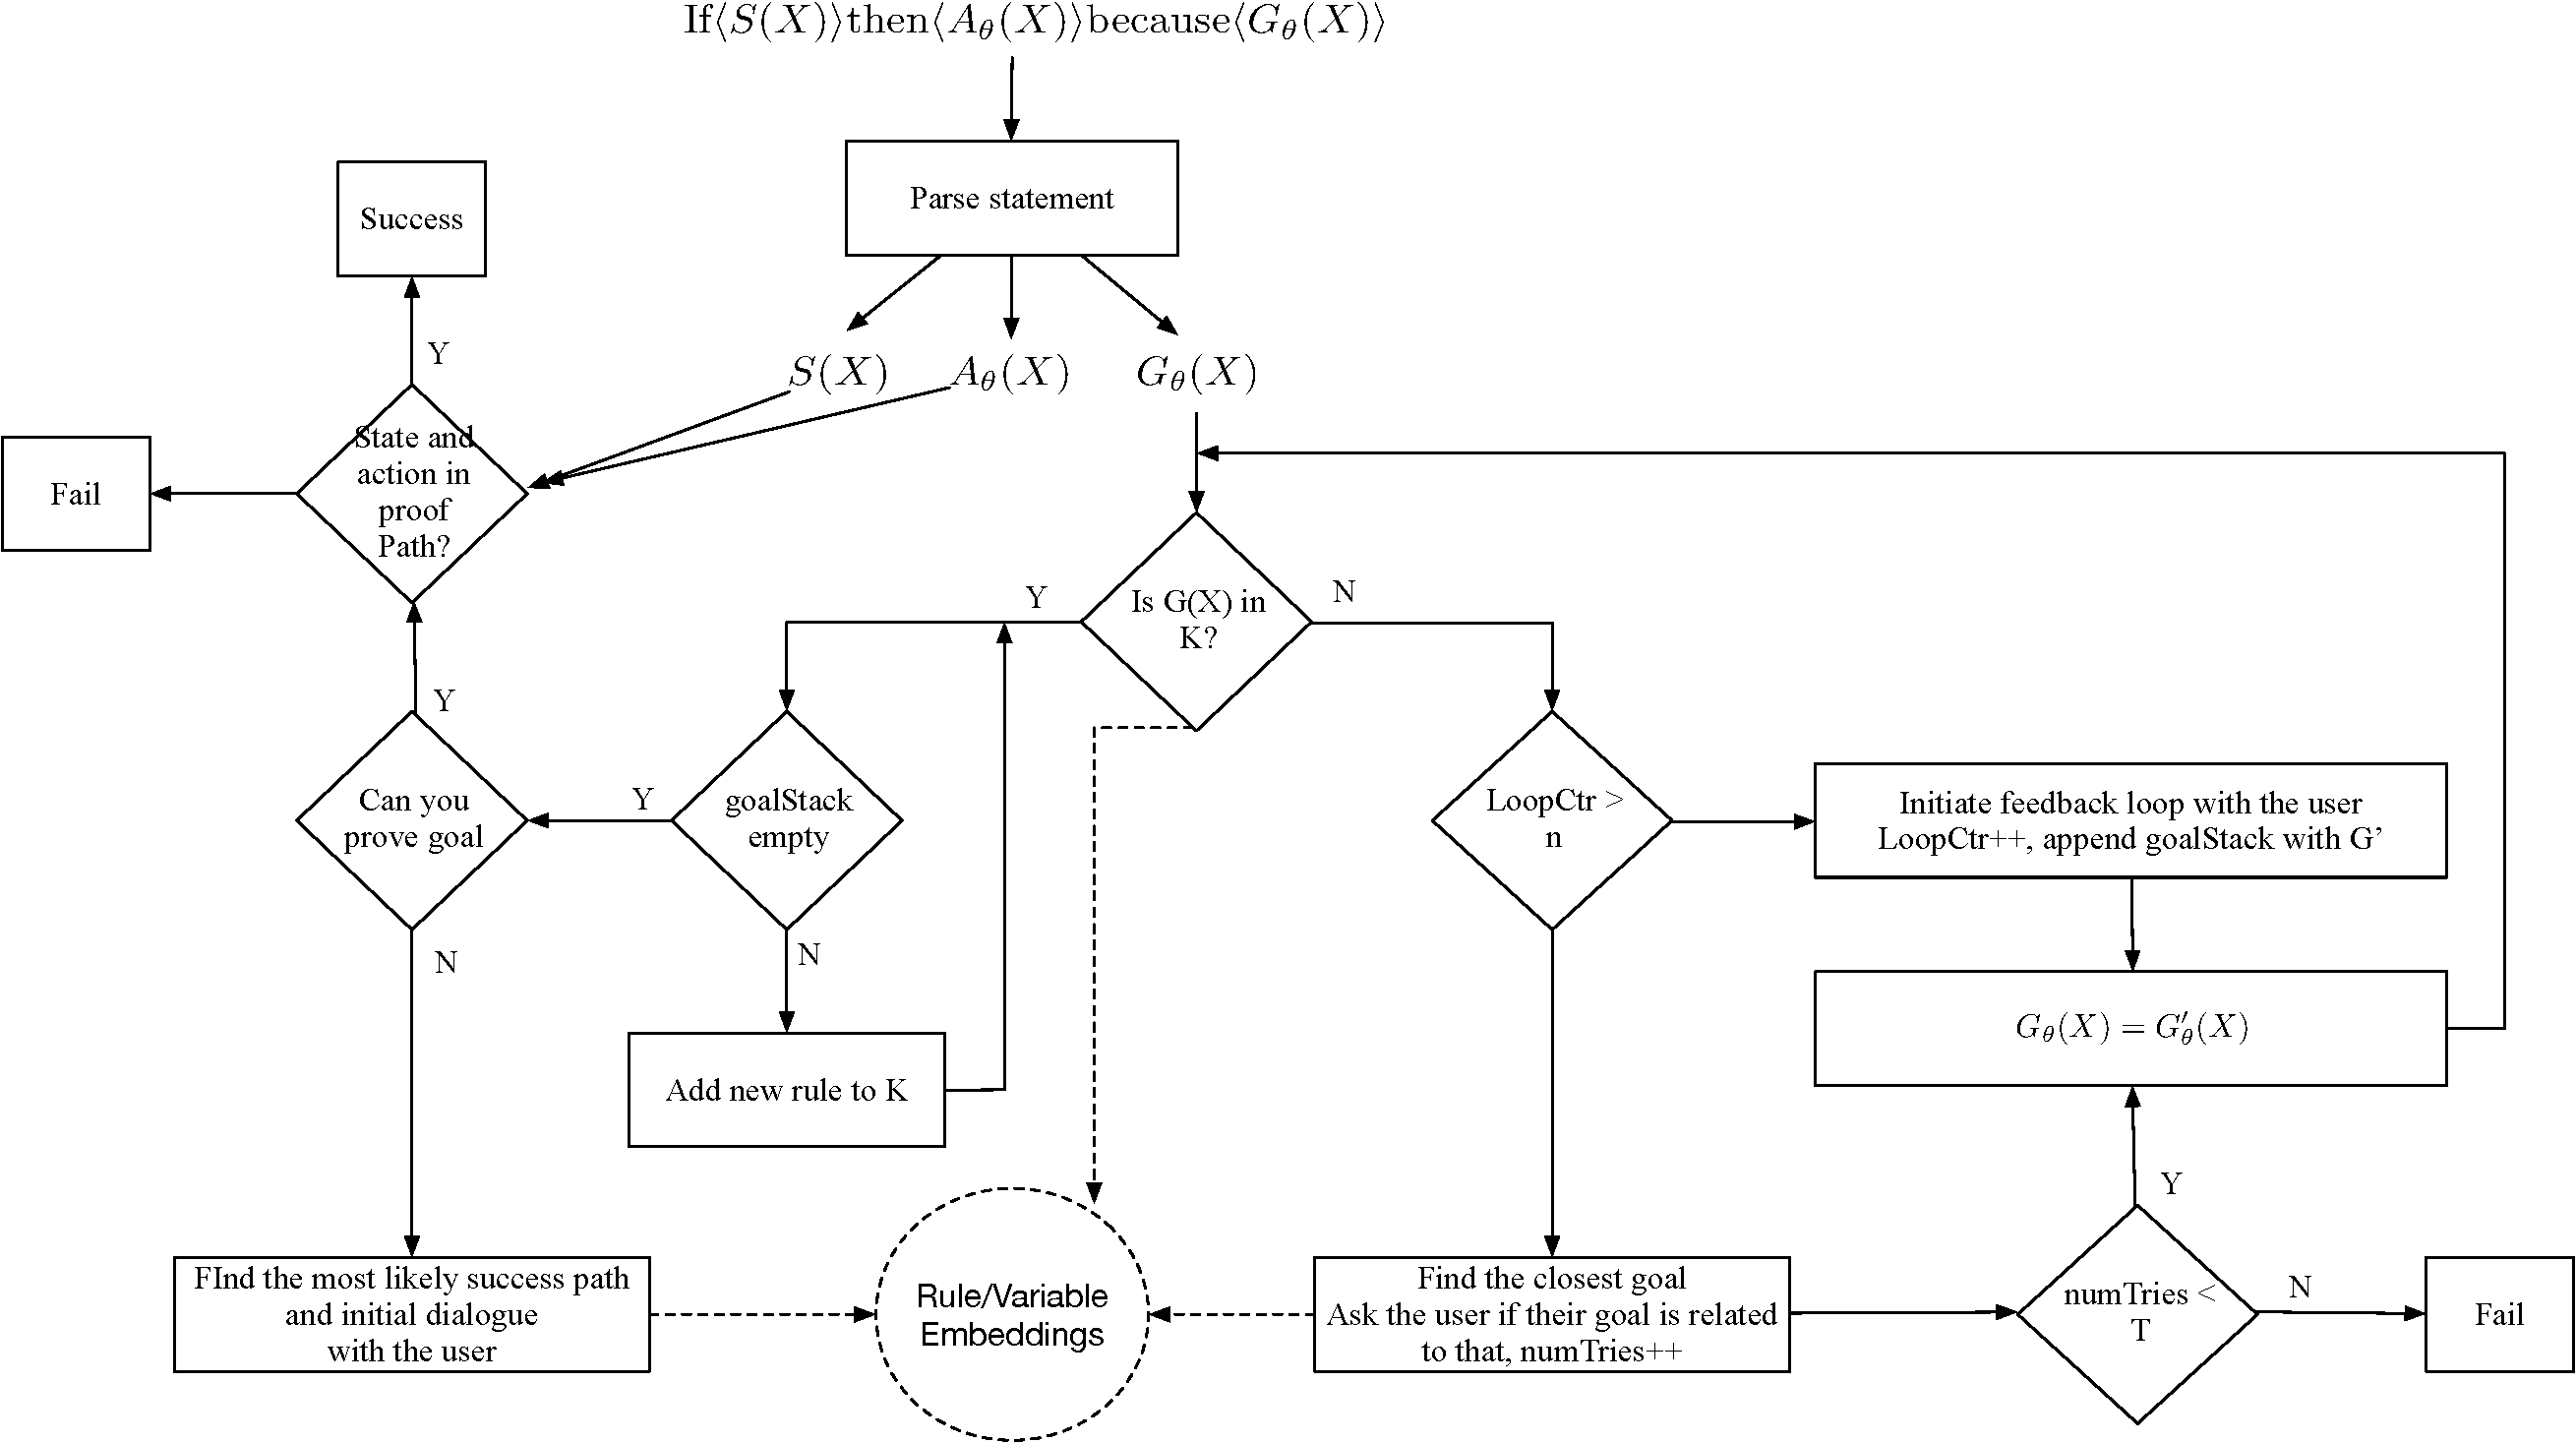
\includegraphics[width=\textwidth]{figs/model.pdf}
    % \caption{Model Architecture \amoscomment{Why 'proposed'? The arrows from S(X) and A(X) make it hard to understand the flow (that is, what happens first, what next). Maybe just remove them or mark it differently (not using arrows).} \facomment{figure is being re-generated}}
    \caption{Model flowchart. $\mathrm{goalStack}$ and the loop variable $i$ are initialized to empty and $0$ respectively. \textcolor{brickred}{Colored text} in the figure represents descriptions.}
    \label{fig:model}
\end{figure}

%These embeddings are used when we need to decide if a rule or a fact is relevant in a proof.
% ``if the forecast is snow tonight'' and ``if the weather is snowy tonight''
% One of the main components of the model is that we learn rule and variable embeddings to combat natural language variations. The main reason for this is that different people have different ways of conveying the same information and the system should be robust to these natural language variations. For example the following two utterances have the same meaning, however, their logical form could be different \amoscomment{I think that we should first define logical form or explain what it is. Especially since you later mention ``predicates".}
% \begin{itemize}
%     \item the weather is rainy tomorrow
%     \item the forecast for tomorrow is rain
% \end{itemize}
% Parsing these two utterances will result in different predicates weather(tomorrow, rainy), forecast(tomorrow, rain). Although these utterances should have the same meaning their predicates have very different forms. Therefore, we propose a model that learns continuous representations for the predicates and logical rules. 
%Before that, let us talk about our parser in more depth in the next subsection.
% We present a learning method that relies on the proof trace of the query to capture the semantic similarity of predicates with different surface forms. 
% In the next two subsections, we present the details of our parser and the model for learning the rule embeddings.

% The dotted lines in Figure \ref{fig:model} indicate the model blocks that rely on the learned embeddings.
% \amoscomment{I don't understand the arrow from Is G(X) in K to "Rule/Variable Embeddings"}

% \facomment{should we address the frame problem here and talk about how it is handled?}